%!TEX root = ../draft.tex
\chapter{Ergebnisse}\label{s.ergebnisse}
Nachdem alle Trainingseinheiten mit den verschiedenen Normalisierungsverfahren durchlaufen wurden, sollen die Ergebnisse aufgeführt und verglichen werden. Zunächst wird die Entwicklungsumgebung beschrieben. Anschließend werden die Ergebnisse untersucht und ausgewertet. 
\section{Frameworks und Entwicklungsumgebung}\label{s.entwicklung}
Wie in vorherigen Kapiteln schon beschrieben, ist das Trainieren eines künstlichen neuronalen Netzes oder eines faltenden neuronalen Netzes sehr rechenintensiv. Die enthaltenen Daten werden parallel mittels Matrizenmultiplikation verarbeitet. Aus diesem Grund werden hauptsächlich Grafikprozessoren für die Verarbeitung verwendet, da diese, im Gegensatz zu normalen Prozessoren, für die Berechnung von Matrizen konzipiert wurden.\\
Auf Softwareseite gibt es eine Menge an Frameworks, mit welchen sich CNNs realisieren lassen. Einige von denen sind beispielsweise Tensorflow, Keras und Theano. Wegen der vorliegenden Erfahrung und der Möglichkeit Trainingsfortschritte grafisch anzeigen zu können, wird der praktische Teil der Arbeit mittels Tensorflow durchgeführt. Tensorflow ist ein Open Source Framework von Google, welches zum Entwickeln von künstlichen neuronalen Netzen genutzt werden kann. Programmiert wurde das Framework in den Programmiersprachen C und Python, welche auch für die Entwicklung genutzt werden. Tensorflow verfügt über eine übersichtliche Dokumentation. Außerdem stehen eine Menge an vortrainierte Netzen als Open Source zur Verfügung. Mithilfe von Tensorboard, welches mit dem Framework zu Verfügung gestellt wird, können die Genauigkeiten eines Netzes erhoben werden. Jede Klasse hat eine eigene durchschnittliche Genauigkeit (AP) und eine Genauigkeit für das gesamte Netz, in Form einer mAP. In den folgenden Tabellen werden bestimmte Abkürzungen wie folgt verwendet: N = Normaler Datensatz, GW = Gray-World-Algorithmus, HA = Histogramm-Ausgleich, HS = Histogramm-Spezifikation (Die besten Ergebnisse einer Klasse wurden durch Rot und Grün hervorgehoben).  
  \section{Nahrungsmittel-Datensatz}
Der erste Datensatz, welcher untersucht wurde ist der Nahrungsmitteltest, der in der Tabelle \ref{tab:nahrungsmitteltest} aufgeführt ist. Dieser enthält, im Vergleich zu den anderen Datensätzen, weniger Objektklassen und weniger Bilder. Außerdem sind die Objekte unter ähnlichen Bedingungen entstanden. Das bedeutet, dass die Lichteinstrahlung in den meisten Fällen ähnlich ist und die Objekte nur in wenigen unterschiedlichen Szenen aufgenommen wurden. In der Tabelle \ref{tab:nahrungsmitteltest} sind die Genauigkeiten des Netzes aufgeführt, welche mit den unterschiedlich behandelten Datensätzen trainiert wurden. Bei genauerer Betrachtung fällt auf, dass kaum nennenswerte Unterschiede bei GW entstanden sind. In manchen Punkten können Verbesserungen in der Genauigkeit ausgewertet werden (Wasser, Orangensaft, Bier), in anderen Punkten wiederum ist die Genauigkeit gesunken(Milch, Brunch, mAP).\\
Bei den Histogramm-Normalisierungen (Ausgleich und Spezifizierung) können größere Unterschiede festgestellt werden. Auch hier sind die Unterschiede in einzelnen Objektklassen besser geworden und in anderen zurückgegangen. Die Genauigkeit der verschiedenen Netze variiert bei dieser hohen Genauigkeit sehr stark, was in der Praxis einen bedeutenden Unterschied machen kann. Insgesamt schneiden die Histogramm-Normalisierungen am schlechtesten ab. Auch ein Blick auf die Datensätze der Histogramm-Normalisierungen zeigt, dass in vielen Fällen Anomalien in den Bildern aufgetreten sind. Gut zu erkennen sind diese in den Abbildungen \ref{img:anoHS} und \ref{img:anoHA}. ???
\begin{table}
[h]
\caption{Durchschnittliche Genauigkeiten des Modells mit dem Nahrungsmittel-Datensatz}
\centering
\begin{tabular}{|l|c|c|c|c|}
\hline
Klassenname & AP(N) & AP(GW) & AP(HA) & AP(HS)\\
\hline
Wasser - Flasche & 0.948 & \textcolor{green}{0.955} & 0.934 & \textcolor{red}{0.917}\\
Orangensaft - Packung & 0.999 & \textcolor{red}{0.998} & \textcolor{green}{1.000} & 0.999\\
Milch - Packung & \textcolor{green}{1.000} & \textcolor{green}{1.000} & \textcolor{green}{1.000} & \textcolor{green}{1.000}\\
Margariene & \textcolor{green}{1.000} & \textcolor{green}{1.000} & \textcolor{green}{1.000} & \textcolor{green}{1.000}\\
Brunch - Aufstrich & \textcolor{green}{1.000} & 0.995 & \textcolor{red}{0.959} & 0.975\\
Flasche - Bier & \textcolor{green}{0.997} & \textcolor{red}{0.970} & 0.986 & 0.979\\
\hline
mAP & \textcolor{green}{0.991} & 0.987 & 0.980 & \textcolor{red}{0.978}\\
\hline
\end{tabular}
\label{tab:nahrungsmitteltest}
\end{table}
\section{PascalVOC Datensatz}
Beim Auswerten der Genauigkeit des normalen Modells fällt auf, dass teilweise große Unterschiede der einzelnen Objektklassen auftreten. Das kann unter anderem daraus resultieren, dass unterschiedlich viele Bilder pro Klasse enthalten sind. Ähnlich wie beim vorherigen Datensatz, konnten zwischen dem originalen Datensatz und der Gray-World-Normalisierung leichte Verluste festgestellt werden. Einige Klassen haben zwar eine höhere durchschnittliche Wahrscheinlichkeit, dennoch gibt es auch hier mehrere Bereiche, in welchen die Genauigkeit abgenommen hat. Auch die mAP hat ca. 0.008 an Genauigkeit verloren. Anders als beim Nahrungsmittel-Datensatz schneidet der Histogramm-Ausgleich weitaus schlechter ab. Nur ein paar Objektklassen konnten besser erkannt werden. Insgesamt verliert das neuronale Netz 0.034 der mAP, was einen gravierenden Unterschied macht. Einige Objektklassen sinken durch die Ausgleichung sogar unter die 50\%-Genauigkeit. Hier wird auch die Schwäche der Histogramm-Spezifikation deutlich. Dadurch, dass keine einheitliche Szene verwendet wurde, sinkt die mAP um 0.045. Die Datensätze haben, im Vergleich zum vorherigen Datensatz, deutlich mehr Anomalien (siehe Abbildung \ref{img:anoHA} und \ref{img:anoHS}).
\begin{table}
[h]
\caption{Durchschnittliche Genauigkeiten des Modells mit dem PascalVOC-Datensatz}
\centering
\begin{tabular}{|l|c|c|c|c|}
\hline
Klassenname & AP(N) & AP(GW) & AP(HA) & AP(HS)\\
\hline
sofa & 0.611 & 0.612 & \textcolor{green}{0.637} & \textcolor{red}{0.602}\\ 
aeroplane & 0.845 & \textcolor{green}{0.855} & \textcolor{red}{0.826} & 0.843\\
horse & \textcolor{green}{0.924} & 0.910 & \textcolor{red}{0.891} & 0.905\\
train & 0.790 & \textcolor{green}{0.804} & \textcolor{red}{0.797} & 0.817\\
bird & \textcolor{green}{0.750} & 0.733 & \textcolor{red}{0.691} & 0.708\\ 
tvmonitor & 0.729 & \textcolor{green}{0.733} & 0.725 & \textcolor{red}{0.691}\\
boat & \textcolor{green}{0.680} & 0.644 & 0.626 & \textcolor{red}{0.559}\\
pottedplant & \textcolor{green}{0.430} & 0.415 & 0.425 & \textcolor{red}{0.340}\\
bus & 0.797 & \textcolor{green}{0.810} & \textcolor{red}{0.763} & 0.776\\ 
diningtable & 0.532 & \textcolor{green}{0.545} & \textcolor{red}{0.507} & 0.517\\
car & 0.812 & \textcolor{green}{0.815} & 0.789 & \textcolor{red}{0.775}\\
bottle & \textcolor{green}{0.553} & 0.510 & 0.498 & \textcolor{red}{0.451}\\
cat & \textcolor{green}{0.903} & 0.902 & 0.872 & \textcolor{red}{0.841}\\
person & \textcolor{green}{0.791} & 0.779 & 0.775 & \textcolor{red}{0.757}\\
chair & 0.499 & \textcolor{green}{0.515} & 0.460 & \textcolor{red}{0.440}\\
bicycle & 0.744 & 0.730 & \textcolor{green}{0.752} & \textcolor{red}{0.697}\\
cow & \textcolor{green}{0.718} & 0.698 & 0.694 & \textcolor{red}{0.653}\\
motorbike & \textcolor{green}{0.739} & \textcolor{red}{0.722} & 0.725 & 0.725\\
dog & \textcolor{green}{0.867} & 0.862 & 0.835 & \textcolor{red}{0.811}\\
sheep & 0.645 & 0.619 & \textcolor{green}{0.664} & \textcolor{red}{0.561}\\
\hline
mAP & \textcolor{green}{0.718} & 0.710 & 0.698 & \textcolor{red}{0.673}\\
\hline
\end{tabular}
\end{table}
  \section{Stanford Dogs Dataset}
Auch bei Überprüfung des dritten Datensatzes fallen ähnliche Muster auf. Der GW-Algorithmus weißt bei diesem Datensatz bessere Ergebnisse auf. Sogar eine Verbesserung gegenüber des originalen Datensatzes konnte erzielt werden. Beim vergleichen der Datensätze fällt auf, dass mehr verschiedene Lichtfarben genutzt wurden, als bei den anderen beiden Datensätzen. Diese konnten vom GW-Algorithmus angepasst werden. Beim Histogramm-Ausgleich und der -Spezifikation wurden, wie auch bei den vorherigen Datensätzen, deutliche Verschlechterungen in der Genauigkeiten festgestellt. Auch hier zeigt einen Blick in die normalisierten Trainingsdaten, dass teilweise starke Farbanomalien aufgetreten sind. Diese behinderten das Training mehr, als das sie hilfreich waren.  
\begin{table}
[h]
\caption{Durchschnittliche Genauigkeiten des Modells mit dem Stanford-Dog-Datensatz}
\centering
\begin{tabular}{|l|c|c|c|c|}
\hline
Objektklasse & AP(N) & AP(GW) & AP(HA) & AP(HS)\\
\hline
Chihuaua & \textcolor{red}{0.729} & \textcolor{green}{0.854} & 0.780 & 0.746\\ 
Shih-Tzu & 0.864 & \textcolor{green}{0.879} & 0.857 & \textcolor{red}{0.832}\\
Rhodesian Ridgeback & \textcolor{green}{0.741} & 0.706 & 0.711 & \textcolor{red}{0.699}\\
Bloodhound & 0.872 & \textcolor{green}{0.878} & 0.904 & \textcolor{red}{0.848}\\
Redbone & \textcolor{green}{0.617} & 0.546 & \textcolor{red}{0.486} & 0.507\\ 
Japanese Spaniel & 0.886 & 0.919 & \textcolor{green}{0.939} & \textcolor{red}{0.837}\\
Blenheim Spaniel & \textcolor{green}{0.980} & 0.966 & 0.944 & \textcolor{red}{0.906}\\
Afghan Hound & \textcolor{green}{0.955} & \textcolor{red}{0.946} & 0.947 & 0.953\\
Bluetrick & \textcolor{green}{0.897} & 0.892 & \textcolor{red}{0.864} & 0.870\\ 
Borzoi & \textcolor{green}{0.931} & \textcolor{red}{0.922} & 0.932 & 0.925\\
Maltese dog & \textcolor{green}{0.905} & 0.901 & \textcolor{red}{0.874} & 0.784\\
Papillon & 0.971 & \textcolor{green}{0.984} & 0.973 & \textcolor{red}{0.952}\\
Basset & 0.763 & \textcolor{green}{0.779} & \textcolor{red}{0.707} & 0.711\\
Coonhound & \textcolor{red}{0.863} & 0.864 & \textcolor{green}{0.895} & 0.901\\
Irish Wolfhound & \textcolor{green}{0.945} & 0.930 & 0.940 & \textcolor{red}{0.905}\\
Pekinese & \textcolor{red}{0.723} & \textcolor{green}{0.840} & 0.743 & 0.782\\
Toy Terrier & 0.838 & \textcolor{green}{0.856} & \textcolor{red}{0.784} & 0.804\\
Beagle & 0.725 & \textcolor{green}{0.743} & \textcolor{red}{0.665} & 0.669\\
Walker Hound & \textcolor{green}{0.767} & \textcolor{red}{0.705} & 0.757 & 0.733\\
Italian Greyhound & 0.822 & \textcolor{green}{0.845} & 0.800 & \textcolor{red}{0.785}\\
\hline
mAP & 0.840 & \textcolor{green}{0.848} & 0.829 & \textcolor{red}{0.807}\\
\hline
\end{tabular}
\end{table}
\section{Zwischenstand}
Um herauszufinden wodurch die abnehmenden Genauigkeiten in der Klassifizierung entstanden sind, wurden die Trainingsdaten überprüft. Dabei ist aufgefallen, dass bei der Histogramm-Ausgleichung und der -Spezifikation große Unterschiede in den Datensätzen vorhanden sind. Das könnte daran liegen, dass die Normalisierung die Farbinformationen des gesamten Bildes nimmt und diese anpasst. Hier macht es einen großen Unterschied, ob die Umgebung in dem Bild hell, dunkel oder eine andere dominante Farbe hat. Bei der Histogramm-Spezifikation kommt zusätzlich noch das Referenzbild hinzu, welches für den Datensatz verwendet wird. Bei der verwendeten Art von Datensätzen, konnte kein einheitliches Referenzbild genutzt werden, da fast jedes Bild unter anderen Bedingungen entstanden ist. Durch diese unterschiedlichen Trainingsbilder kommt es zu Anomalien in den normalisierten Bildern (Abbildung \ref{img:evalHA}). Um diese Vermutung zu bestärken, wurden Objekte mit gleicher Lichteinstrahlung und gleicher Entfernung auf unterschiedlichen Hintergründen aufgenommen (Abbildung \ref{img:evalnorm}). Daraufhin wurden die Bilder jeweils mit allen Verfahren normalisiert. Das Objekt auf dem Bild wurde vom Hintergrund segmentiert, um zu überprüfen, wie sich die Histogramme des Objektes voneinander unterscheiden. (Abbildung \ref{img:evalHA}).\\
\begin{figure}[htb]
\begin{minipage}[c]{0.2\textwidth}
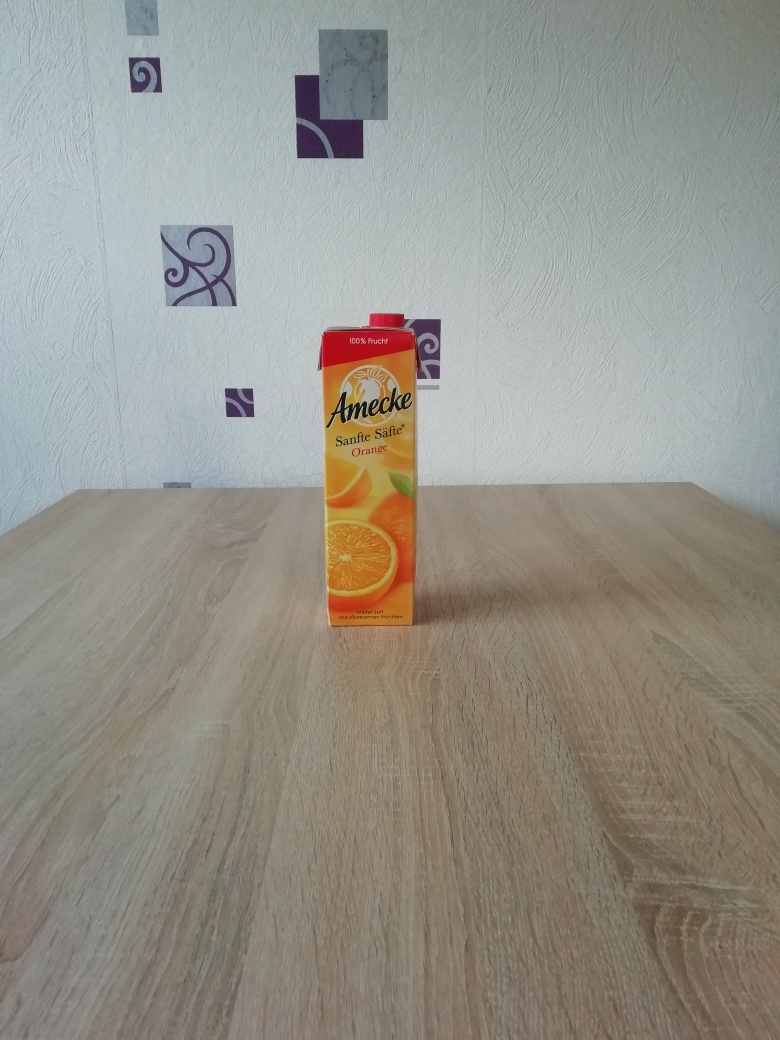
\includegraphics[width=\textwidth]{Sources/Bild1.jpg}
\end{minipage}
\hfill
\begin{minipage}[c]{0.08\textwidth}
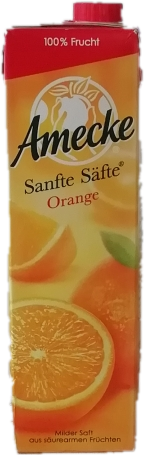
\includegraphics[width=\textwidth]{Sources/Bild1.png}
\end{minipage}
\hfill
\begin{minipage}[c]{0.3\textwidth}
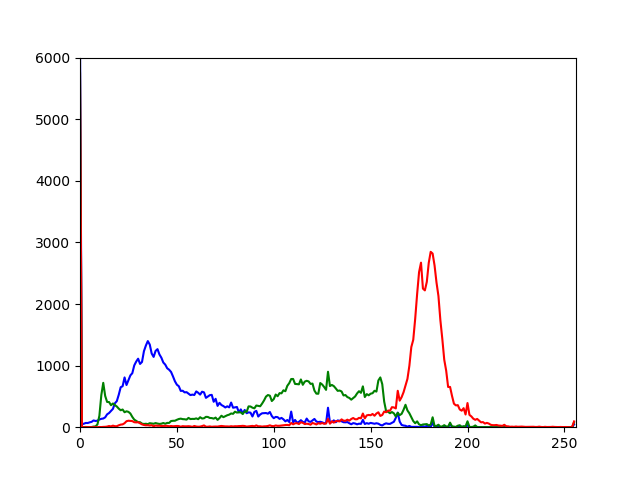
\includegraphics[width=\textwidth]{Sources/Bild1_histo.png}
\end{minipage}
\end{figure}
\begin{figure}[htb]
\begin{minipage}[c]{0.2\textwidth}
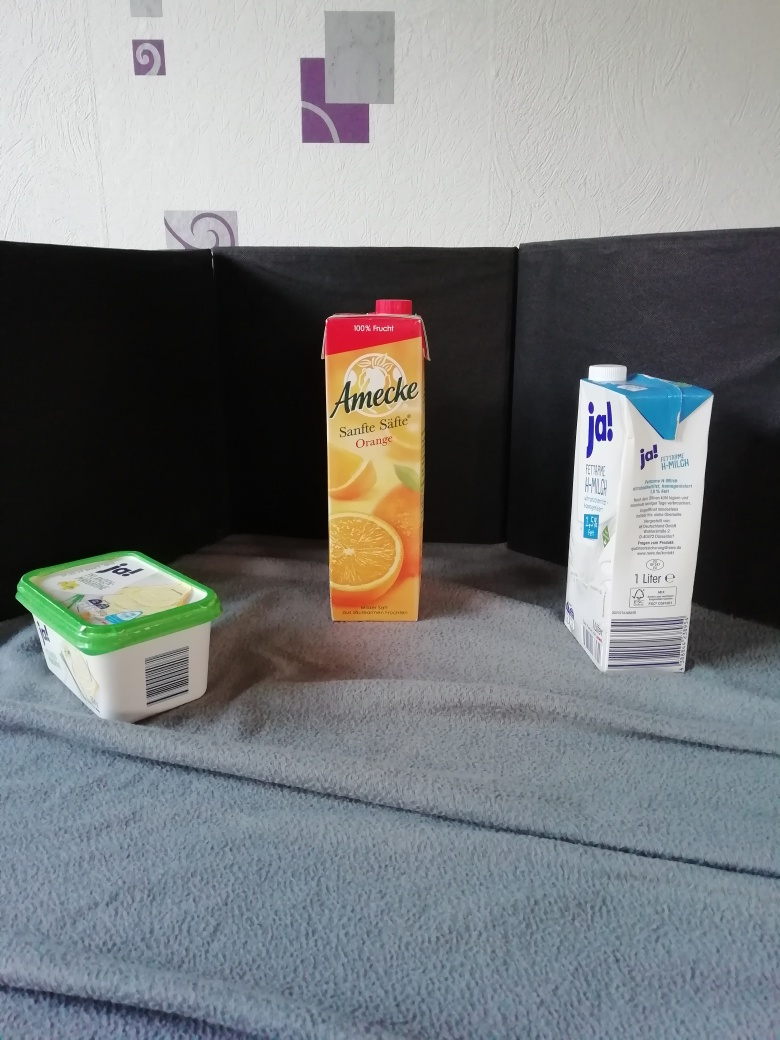
\includegraphics[width=\textwidth]{Sources/Bild2.jpg}
\end{minipage}
\hfill
\begin{minipage}[c]{0.08\textwidth}
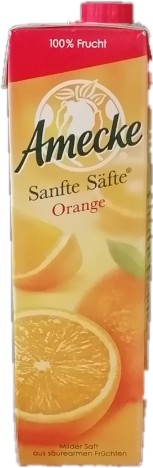
\includegraphics[width=\textwidth]{Sources/Bild2.png}
\end{minipage}
\hfill
\begin{minipage}[c]{0.3\textwidth}
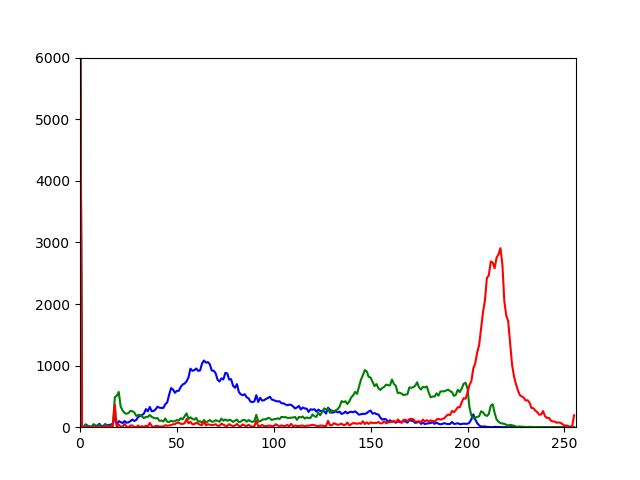
\includegraphics[width=\textwidth]{Sources/Bild2_histo.png}
\end{minipage}
\caption{Histogramm des segmentierten Objektes aus dem Nahrungsmittel-Datensatz ohne Normalisierung}
\label{img:evalnorm}
\end{figure}\\
Durch diesen Test wurde bestätigt, dass die Ergebnisse der Histogramm-Ausgleichung und -Spezifikation sehr unterschiedlich geworden sind. Die Veränderung des Umfeldes beeinflusst also das Ergebnis entscheidend und sorgt für größere Farbveränderungen, als der Lichteinfluss selbst.
Ein Datensatz mit einheitlichem Hintergrund in den Trainingsdaten, könnte mit den Normalisierungsverfahren besser funktionieren. Um diese Annahme weiter überprüfen zu können, soll ein weiterer Datensatz generiert werden, in dem ein einheitlicher Hintergrund festgelegt ist. 
\section{Obst-Datensatz}
Für einen weiteren Versuch wurde der Obstdatensatz erstellt. Dieser besteht aus den Objekten, welche in Tabelle \ref{tab:obst} aufgelistet sind. Bei diesem Datensatz wurde darauf geachtet einen einheitlichen Hintergrund zu verwenden, um die Funktionalität bei anderen Einstellungen zu testen. Außerdem wurde, im Vergleich zum Nahrungsmittel Datensatz (Tabelle \ref{tab:nahrungsmittel}), darauf geachtet, ähnlichere Klassen zu verwenden, auf welchen optimalerweise keine Schrift enthalten ist. Das Netz soll nicht durch die Schrift beeinflusst werden, sondern hauptsächlich die Farben als Orientierung nehmen.
\begin{table}[htb]
\caption{Klassen des Obst-Datensatzes mit konstantem Hintergrund}
\center
\begin{minipage}[c]{.4\textwidth} 
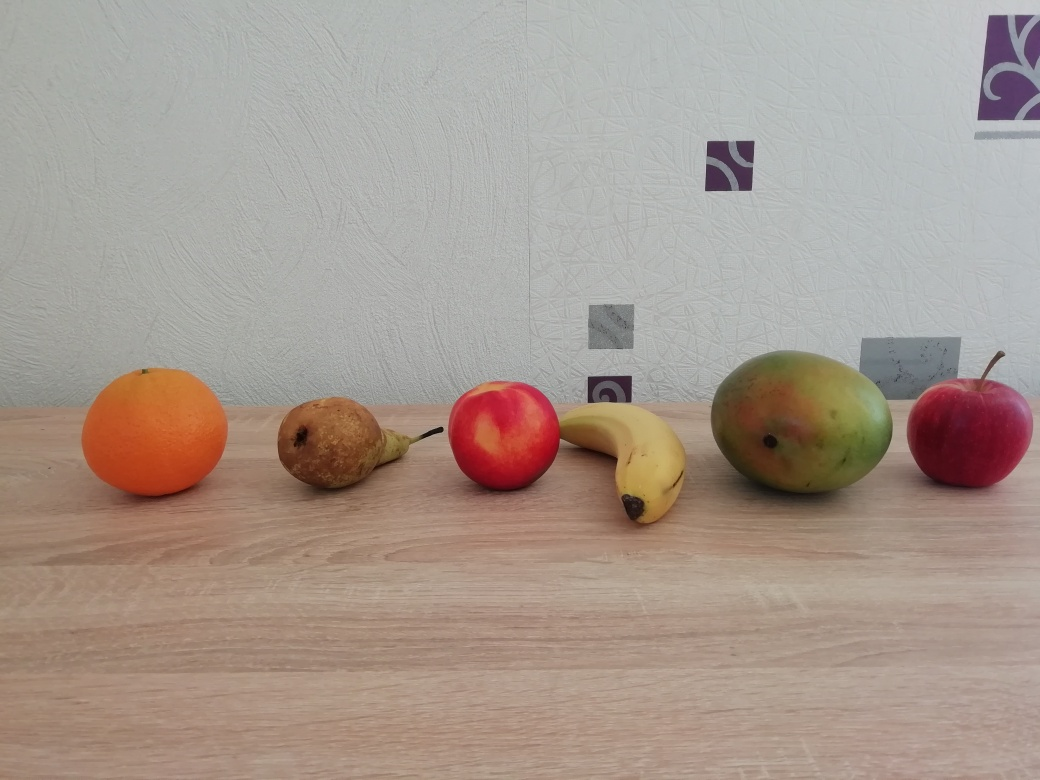
\includegraphics[width=.8\textwidth]{Sources/Obst_mit_hintergrund}  
\end{minipage} 
\begin{minipage}[c]{.4\textwidth}\label{tab:obst}   
\begin{tabular}{|l|l|}
\hline
Klassenname & Klassenname\\
\hline
Orange & Mango\\
Banane & Nektarine\\
Apfel & Birne\\
\hline
\end{tabular} 
\end{minipage}
\end{table}  
Dieser Datensatz wird, genau wie die vorherigen Datensätze, mit den unterschiedlichen Methoden normalisiert. Dabei soll zum einen die Genauigkeit der einzelnen Klassen betrachtet werden und zum anderen die Trainingsdaten an sich. Hierbei soll überprüft werden, ob die Trainingsbilder wie erwartet aussehen und wie stark Anomalien auftreten. 
\section{Auswertung des Obst-Datensatzes}
Nach Auswertung der Trainingsergebnisse kann festgestellt werden, dass zwei der drei Normalisierungsmethoden einen positiven Einfluss auf die Klassifizierung haben. 
Die Genauigkeit der Histogramm-Spezifikation schneidet mit 97\% am besten ab. Durch diese Methode konnte eine Erhöhung von 43\% erzielt werden. Auch der Gray-World-Algorithmus hat eine leichte Verbesserung von 14\% bewirkt. Lediglich der Histogramm-Ausgleich hat die Klassifizierung leicht verschlechtert. Eine weitere Möglichkeit den Einfluss zu überprüfen wurde mit Hilfe von besonders schwierigen Testbildern versucht. Dafür sollen Bildaufnahmen mit extremen unterschiedlichen Lichteinflüssen verwendet werden.
\begin{table}
[h]
\caption{Genauigkeitsberechnungen des Modells des Obst-Datensatzes}
\centering
\begin{tabular}{|l|c|c|c|c|}
\hline
Klassenname & AP(N) & AP(GW) & AP(HA) & AP(HS)\\
\hline
Orange & \textcolor{red}{0.982} & 0.985 & 0.983 & \textcolor{green}{1.000}\\
Nektarine & \textcolor{red}{0.986} & 0.988 & \textcolor{green}{0.993} & 0.987\\
Banane & \textcolor{green}{1.000} & \textcolor{green}{1.000} & \textcolor{green}{1.000} & \textcolor{green}{1.000}\\
Mango & 0.993 & 0.996 & \textcolor{red}{0.983} & \textcolor{green}{1.000}\\
Apfel & 0.995 & 0.996 & \textcolor{red}{0.990} & \textcolor{green}{0.999}\\
Birne & 0.999 & \textcolor{red}{0.998} & \textcolor{green}{1.000} & \textcolor{green}{1.000}\\
\hline
mAP & 0.993 & 0.994 & \textcolor{red}{0.992} & \textcolor{green}{0.997}\\
\hline
\end{tabular}
\end{table}
Die Auswertung der normalisierten Trainingsdaten hat ergeben, dass wesentlich weniger Farbanomalien auftreten, als bei den vorherigen Datensätzen. Dabei ist aufgefallen, dass gerade bei den Histogramm-Normalisierungen mit einheitlichem Hintergrund deutliche Verbesserungen erzielt wurden. Große Veränderungen treten nur dann auf, wenn viele Objekte auf dem Bild enthalten sind, da diese die Umgebung zu stark beeinflussen oder bei der Histogramm-Ausgleichung, wenn die Beleuchtung zu extrem verändert wurde. Die Histogramm-Spezifikation geht mit diesem Problem am besten um, weil sie ein Referenz-Histogramm verwendet, um die Daten anzupassen. \\\\
Auch die Helligkeitsverteilungen der Trainingsdaten werden wesentlich besser, wie in den Beispielen in der Abbildung \ref{img:hellver} zu erkennen ist. Dafür wurde eine stark unterbelichtete Aufnahme generiert, um die Veränderung nach den Normalisierungsmethoden besser herauszustellen. Die beste Helligkeitsverteilung konnte dabei der Histogramm-Ausgleich aufweisen, wobei durch das dunkle Quellbild die Farbinformationen zum großen Teil verloren gegangen sind. Der Gray-World-Algorithmus hat die Helligkeitsverteilung kaum verändert, was daran liegt, dass die Farbverteilung durch die Höhe des Grünkanals verschoben wird und nicht für solche Aufgaben ausgelegt ist. Das insgesamt beste Ergebnis liefert die Histogramm-Spezifikation. Nicht nur die Helligkeitsverteilung konnte verbessert werden, auch die Farben konnten vergleichsweise gut wieder hergestellt werden.
